\documentclass[CJK]{beamer}
\usepackage{CJKutf8}
\usepackage{beamerthemesplit}
\usetheme{Malmoe}
\useoutertheme[footline=authortitle]{miniframes}
\usepackage{amsmath}
\usepackage{amssymb}
\usepackage{graphicx}
\usepackage{color}
\usepackage{slashed}
\usepackage{simplewick}
\graphicspath{{../figures/}}
\def\be{\begin{equation}}
\def\ee{\nonumber\end{equation}}
\def\bea{\begin{eqnarray}}
\def\eea{\nonumber\end{eqnarray}}
\def\ii{{\dot{\imath}}}
\def\bch{\begin{CJK}{UTF8}{gbsn}}
\def\ech{\end{CJK}}
\def\bex{\begin{minipage}{0.3\textwidth}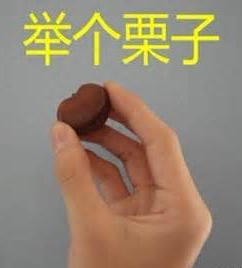
\includegraphics[width=1in]{jugelizi.png}\end{minipage}\begin{minipage}{0.6\textwidth}}
\def\eex{\end{minipage}}
\def\chtitle#1{\frametitle{\bch#1\ech}}
\def\skipline{{\vskip0.1in}}
\def\skiplines{{\vskip0.2in}}
\def\lagr{{\mathcal{L}}}
\def\hamil{{\mathcal{H}}}
\def\vecv{{\mathbf{v}}}
\def\vecx{{\mathbf{x}}}
\def\veck{{\mathbf{k}}}
\def\vecp{{\mathbf{p}}}
\def\vecn{{\mathbf{n}}}
\def\vecA{{\mathbf{A}}}
\def\vecP{{\mathbf{P}}}
\def\vecsigma{{\mathbf{\sigma}}}
\def\hatJn{{\hat{J_\vecn}}}
\def\hatJx{{\hat{J_x}}}
\def\hatJy{{\hat{J_y}}}
\def\hatJz{{\hat{J_z}}}
\def\hatj#1{\hat{J_{#1}}}
\def\hatphi{{\hat{\phi}}}
\def\hatq{{\hat{q}}}
\def\hatpi{{\hat{\pi}}}
\def\vel{\upsilon}
\def\Dint{{\mathcal{D}}}
\def\adag{{\hat{a}^\dagger}}
\def\bdag{{\hat{b}^\dagger}}
\def\cdag{{\hat{c}^\dagger}}
\def\ddag{{\hat{d}^\dagger}}
\def\hata{{\hat{a}}}
\def\hatb{{\hat{b}}}
\def\hatc{{\hat{c}}}
\def\hatd{{\hat{d}}}
\def\hatN{{\hat{N}}}
\def\hatH{{\hat{H}}}
\def\hatp{{\hat{p}}}
\def\Fup{{F^{\mu\nu}}}
\def\Fdown{{F_{\mu\nu}}}
\def\newl{\nonumber \\}
\def\SIkm{\mathrm{km}}
\def\SIyr{\mathrm{yr}}
\def\SIGyr{\mathrm{Gyr}}
\def\SIeV{\mathrm{eV}}
\def\SIGeV{\mathrm{GeV}}
\def\SIm{\mathrm{m}}
\def\SIcm{\mathrm{cm}}
\def\SIJ{\mathrm{J}}
\def\SIs{\mathrm{s}}
\def\SIkg{\mathrm{kg}}
\def\SIg{\mathrm{g}}
\def\vece{\mathrm{e}}
\def\bmat#1{\left(\begin{array}{#1}}
\def\emat{\end{array}\right)}
\def\bcase#1{\left\{\begin{array}{#1}}
\def\ecase{\end{array}\right.}
\def\calM{{\mathcal{M}}}
\def\calT{{\mathcal{T}}}
\def\calR{{\mathcal{R}}}
\def\barpsi{\bar{\psi}}
\def\baru{\bar{u}}
\def\barv{\bar{\upsilon}}
\def\bmini#1{\begin{minipage}{#1\textwidth}}
\def\emini{\end{minipage}}
\def\qeq{\stackrel{?}{=}}
\def\torder#1{\mathcal{T}\left(#1\right)}
\def\rorder#1{\mathcal{R}\left(#1\right)}


\title{Quantum Field Theory I \\ Lesson 02 - Action Princple}
  \author{}
  \date{}


\begin{document}

\begin{frame}
 
\begin{center}
\begin{Large}
\bch
量子场论 I 

{\vskip 0.3in}

第二次课后作业 (共八次,每次2.5分)

交作业时间: 10月10日,星期一,13:30pm

\ech
\end{Large}
\end{center}

\vskip 0.2in

\bch
课件下载
\ech
https://github.com/zqhuang/SYSU\_QFTI

\end{frame}

\begin{frame}
\chtitle{第1题(0.5分)}
\bch
对质量为$m$的自由实标量场$\phi$,四维动量$k$满足$k^0 = \omega \equiv \sqrt{\veck^2+m^2}$,其中$\veck\equiv (k^1, k^2, k^3)$为三维动量。对任意洛仑兹变换下不变的函数$f(k)$,证明积分$\int \frac{d^3\veck}{2\omega} f(k)$ 也是洛仑兹变换下的不变量。
\ech
\end{frame}

\begin{frame}
\chtitle{第2题(0.5分)}
\bch
对质量为$m$的自由实标量场$\phi$,证明四维时空下的任意两点场算符的对易$[\hatphi(x),\hatphi(x')]$是洛仑兹变换下的不变量。(提示:利用$\hatphi$的算符表达式和第1题结论。)
\ech
\end{frame}

\begin{frame}
\chtitle{第3题(0.5分)}
\bch
质量为$m$的自由复标量场,
$$\langr = \partial_\mu\phi^\dagger \partial^\mu \phi - m^2\phi^\dagger\phi\, $$
把$\phi$和$\phi^\dagger$分别看作独立自由度,它们对应的正则动量分别为
$$\pi = \frac{\partial \langr}{\partial \dot\phi} = \dot\phi^\dagger, \,\pi^\dagger = \frac{\partial \langr}{\partial \dot\phi^\dagger} = \dot\phi $$
于是Hamilton密度为
$$\hamil = \dot\phi^\dagger \pi^\dagger +\dot\phi \pi - \langr = \pi^\dagger \pi + \nabla\phi^\dagger \cdot\nabla\phi + m^2\phi^\dagger \phi $$
我们在课堂上推到了量子化后的$\phi$为
$$\hatphi(x) = \frac{1}{(2\pi)^{3/2}} \int \sqrt{\frac{d^3\veck}{2\omega}} \left(\hata_{\veck} e^{-ik_\mu x^\mu} + \bdag_{\veck}e^{ik_\mu x^\mu}\right) $$
试求量子化后的总Hamilton量$\hat{H}$.
\ech
\end{frame}


\begin{frame}
\chtitle{第4题(0.5分)}
\bch
考虑和规范场耦合的复标量场的拉氏密度:
$$\langr = (D^\mu\phi)^\dagger D_\mu \phi - m^2\phi^\dagger \phi  - \frac{1}{4}\Fup\Fdown$$
利用Euler-Lagrange方程
$$\partial_\mu \Fup = j^\nu$$
证明$j_\mu$是守恒流.
\ech
\end{frame}


\begin{frame}
\chtitle{第5题(0.5分)}
\bch
关于三维空间转动算符
\begin{itemize}
\item{证明相反方向的角动量算符相差一个负号$\hat{J}_{-\vecn} = - \hatJn$}
\item{因为绕固定轴转动$2\pi$的没有任何效果,所以转动算符$e^{-2\pi\ii\hatJn}=1$,由此证明$\hatJn$的本征值一定是整数。}
\item{三个形成右手正交系的方向$\vecn_1$, $\vecn_2$, $\vecn_3$,对应的转动算符分别为$\hatj{1} $, $\hatj{2} $, $\hatj{3}$,证明$\hatj{1}^2+\hatj{2}^2+\hatj{3}^2 = 2$。.}
\end{itemize}
\ech
\end{frame}


\end{document}
